\chapter{Microservice Architecture}
\label{cha:Microservice_Architecture}
This chapter introduces the microservice architecture concepts, which are necessary to understand why the later discussed approaches are needed.
The principles used to design microservices lead to some characteristics, resulting in the motivations and challenges declared in this chapter.
Furthermore some recommendations about the use cases of the microservice architecture are provided and the caused security consequences are declared.

\section{Motivation}
Companies like Netflix, Amazon, and Uber are front-runners for building software solutions using the microservice architecture~\cite{dias2020microservices}.
The main idea is to split the business logic of an application into small autonomous services that work together.
This means the programmers have to avoid the temptation of developing too large systems.
This approach results in the following benefits~\cite{newman2021building}: 
\begin{itemize}
    \item Technology heterogeneity is achieved through the possibility to use different technology stacks for different services, depending on the needs of the services.
		It is even possible to use different data storage for the different microservices (e.g., graph database for users).
    \item Resilience is achieved since component failures can be isolated, so the rest of the system can carry on working by degrading the functionality of the system. 
    \item Scaling is much more effective due to the possibility to scale only the parts of the system that really need scaling.
    \item The deployment is much more convenient because a single microservice can be deployed instead of deploying the whole application, even for small changes.
    \item The organizational alignment can be improved by assigning the work to small teams that work on smaller codebases, resulting in higher productivity.
    \item Composability is achieved, considering that the functionalities can be consumed in different ways for different purposes.
    \item Replaceability is optimized since rewriting a tiny service is much more manageable than replacing a few parts of a vast application.
\end{itemize}

\section{Comparison to the Monolithic Architecture}
\begin{figure}
    \centering
    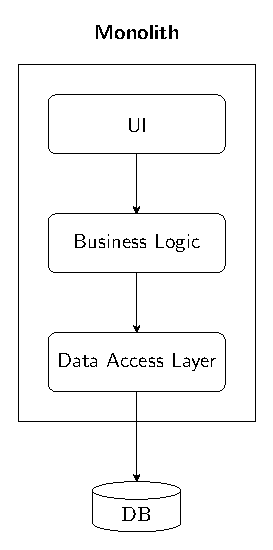
\includegraphics[width=0.3\textwidth]{./images/microservice_architecture/TikZ_Monolith.pdf}
    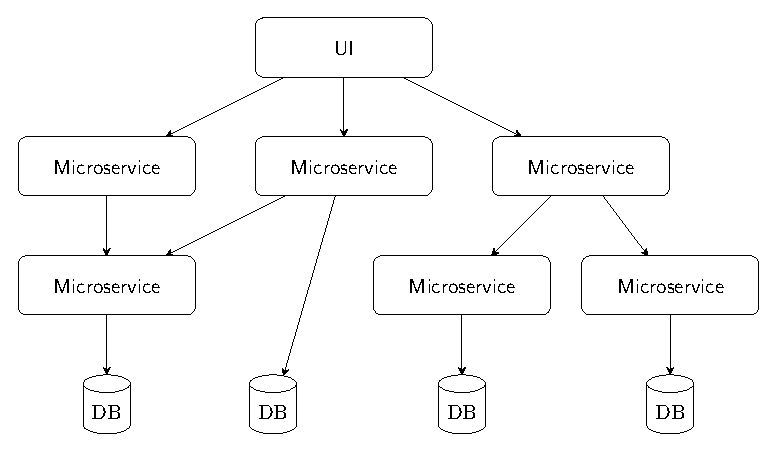
\includegraphics[width=0.69\textwidth]{./images/microservice_architecture/TikZ_Microservice.pdf}
    \caption{Example of monolithic architecture and a microservice architecture~\cite{kalske2017challenges}}
    \label{fig:monolithvsmicroservice}
\end{figure}

Figure~\ref{fig:monolithvsmicroservice} shows the architectural differences between monolithic and microservice applications.
A monolithic application has a single unit containing the user interface layer (UI), the business logic layer, and the data access layer.
Therefore it is much simpler to manage but brings the following downsides regarding the codebase~\cite{kalske2017challenges}:
\begin{itemize}
    \item New features and modifications of old features are harder to implement.
    \item Refactoring changes can reflect many parts of the software
    \item Code duplication raises since it is almost impossible to reuse existing code
\end{itemize}
The microservice architecture consists of multiple services focused on only one function of the business logic.
Those services communicate with other services using remote calls (e.g., over HTTP), which causes higher latencies.
Depending on the needs of the services, each service can have its own database, which can differ from the database system of the other services.
It is also possible to share one database for multiple services, but this should be avoided to reduce coupling between the services. 

\section{Design Principles}
It is hard to define principles, which will apply to all microservice architectures, but according to Newman, most of them will adhere to the following principles~\cite{newman2021building}: 
\begin{description}
    \item[Modelled around business concepts:] The functionalities are structured around the business contexts instead of the technical concepts.
    \item[Adopting culture of automation:] The microservice deployments embrace the culture of automation by using automated tests, continuous delivery, automated servers, and much more automation tools.
    \item[Hiding implementation details:] The microservices hide as many implementation details as possible to avoid coupling.
		Especially the databases of the services should be hidden and can be accessed by other services using APIs.
    \item[Decentralising all The things:] All approaches that could centralize business logic are avoided to keep associated data and logic within the service boundaries.
    \item[Independently deployed:] The microservices should provide the possibility to deploy them without having to deploy any other service.
		Therefore the autonomy of the teams can be increased, and new features can be released faster.
    \item[Isolates failures:] The microservices have to deal with misbehaving parts of the system and keep on providing as much functionality as possible, to prevent cascading failure.
    \item[Highly observable:] It is not sufficient to observe a single service's behavior and status.
		Instead, the functioning of the whole system has to be monitored.
\end{description}

\section{Challenges} \label{sec:microservice_challenges}
There are some benefits of using the microservice architecture.
It also introduces a set of challenges, which could argue to avoid the microservice architecture in some cases.
According to Kalske et al.~\cite{kalske2017challenges} the microservice architecture brings the following technical challenges with it: 
\begin{itemize}
    \item The declaration of the service boundaries is very hard~\cite{kalske2017challenges}, especially if the developers do not know the domain that well~\cite{newman2021building}.
    \item The services should not become too fine-grained to prevent performance overhead.
		Otherwise, if they are not decomposed enough, changes to one service can affect multiple services.
    \item Continuous Delivery and Continuous Integration are  necessary to manage the services and validate their functionality.
    \item The integration of the services into other services can become very hard due to the requirement to be available for all used technologies.
    \item Good logging mechanisms have to be used to recognize failures of microservices as soon as possible.
    \item Fault tolerance mechanisms have to be implemented to react to situations in which needed services do not respond.
\end{itemize}
The microservice architecture is gaining popularity, even if it produces so many challenges, showing how crucial its advantages are.

\section{Usage Situation}
According to Newman~\cite{newman2021building} it is better to start with a monolithic application if the architect does not fully understand the domain and has problems declaring the boundaries for the services.
In such cases, it is better to spend some time learning what the system does first and then break things down to microservices when the system is stable.
Furthermore, Newman recommends eliminating legacy monitoring systems before splitting the application into more and more microservices.
Otherwise, it could get very messy to stay in knowledge about the system's status.

Fowler~\cite{fowlerpremium} recommends considering microservices only when a system gets too complex to manage as a monolith.
His essence is keeping the system simple enough to avoid the need of microservices since the microservice architecture can slow down the development considerably.
The correlation between the development productivity and the complexity of a system comparing the microservice architecture with a monolithic architecture is shown in figure~\ref{fig:fowler_productivity}.

\begin{figure}[H]
    \centering
    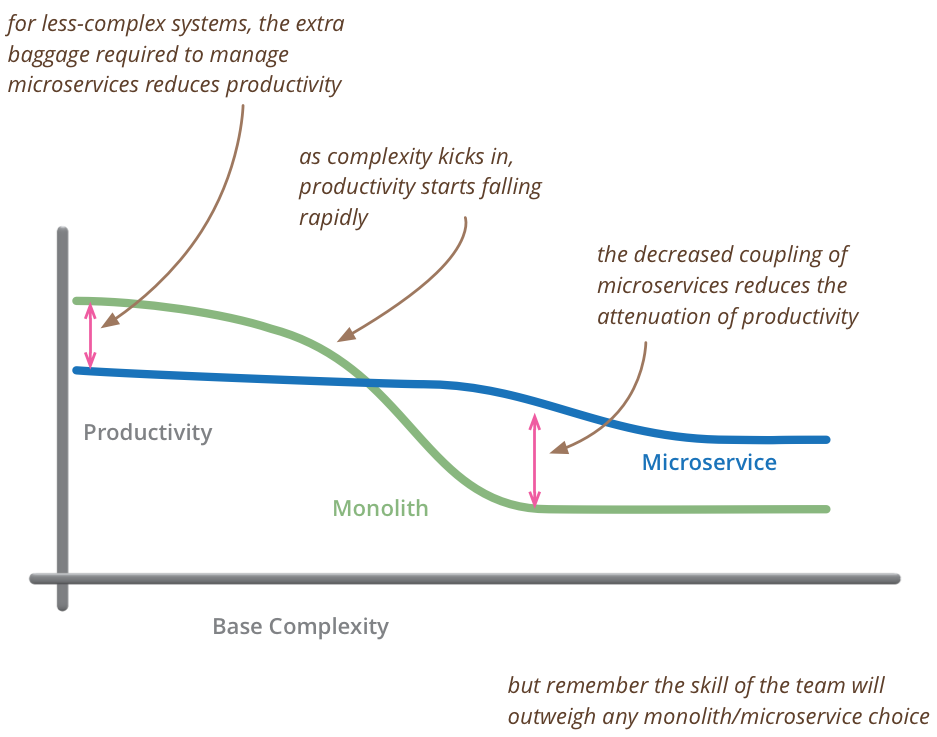
\includegraphics[width=0.7\textwidth]{./images/microservice_architecture/fowler-productivity-complexity.png}
    \caption{Correlation between base complexity and productivity in a microservice architecture compared to a monolithic architecture~\cite{fowlerpremium}}
    \label{fig:fowler_productivity}
\end{figure}

\section{Security Consequences}
The migration to the microservice architecture brings many consequences regarding the security of a deployment.
Especially the network communications among the services introduce a set of vulnerabilities.
Confidentiality, integrity, and availability have to be assured.
The need for authentication mechanisms is a common issue of network security, but the migration from language-level calls to remote calls causes the need for authentication between microservices.
Therefore, the authentication mechanisms discussed in this thesis are a consequence of the microservice architecture and can be neglected with a monolithic architecture.
